\documentclass[aspectratio=149, ] {beamer}
%\usepackage[latin1]{inputenc}    
\usecolortheme{crane}
\usepackage[crane]{katescodingstyles}

\usepackage{pgfpages}






\newcommand{\pyTWO}[1][]{
  \begin{tikzpicture}[remember picture,overlay,#1]
    \node {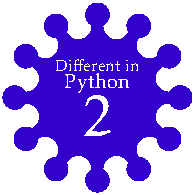
\includegraphics[scale=.5]{pyTWO}};
  \end{tikzpicture}% 
}

\setbeamertemplate{navigation symbols}{}


\begin{document}


\begin{frame}[fragile]{One more method\dots maybe an attribute?}
  
  Suppose we need the length of the diagonal of our rectangle.
  
  \pause \smallskip
  
  Since the diagonal of a rectangle with sides $l$ and $w$ 
  is $\sqrt{l^2 + w^2}$,\\[-1pt]
  we can write a method:
  
  \smallskip \pause
   
  \only<3|handout:0>{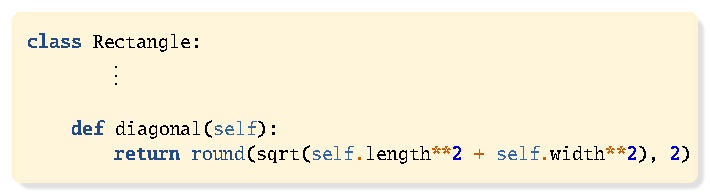
\includegraphics[page=1]{diagonal}}
  \onslide<4->
  \includegraphics[page=2]{diagonal}
  
  The \inline`@property` decorator makes a method seem like an
  attribute.
  
  
\end{frame}





\end{document}